\section{Конструкторская часть}

В данном разделе будут сформулированы требования и ограничения к разрабатываемому методу. 
Разработан метод динамического отображения изменений пользовательского интерфейса на основе обработки изменений XML--файла.
Описаны основные этапы разработки в виде детализированной диаграммы IDEF0 и схем алгоритмов, а также изложены особенности излагаемого метода. 

\subsection{Требования и ограничения к разрабатываемому методу}

К методу динамического отображения изменений пользовательского интерфейса на основе обработки изменений XML--файла предъявляются следующие требования:
\begin{enumerate}
	\item Обработка события, инициирующего изменения интерфейса во время выполнения.
	\item Преобразование XML-файла, организованного определенным образом, в UI-элементы.
	\item Размещение UI-элементов на экране.
\end{enumerate}
	
Также представлено ограничение для разрабатываемого метода: при неправильной организации XML--файла не гарантируется корректное отображение элементов на экране.


%Ниже приведено описание каждой из функций, представленных на рисунке \ref{fig:zram-archeticture}:


\subsection{Требования к разрабатываемому программному обеспечению}

К разрабатываемому программному обеспечению предъявляются следующие требования:
\begin{enumerate}
	\item Возможность обработки события, инициирующего изменение интерфейса.
	\item Возможность во время выполнения программы изменять интерфейс посредством внесения изменения в XML--файл по срабатыванию обработчика события.
	\item Возможность создавать интерфейсы с вложенностью элементов.
	\item Возможность создавать интерфейсы со всеми базовыми UI--элементами.
	\item Возможность оперировать базовыми параметрами UI--элементов.
	\item Возможность комбинировать существующие методы создания интерфейса с разрабатываемым.
	\item Разрабатываемое ПО должно корректно реагировать на любые действия пользователя.
\end{enumerate}

\subsection{Основные этапы разрабатываемого метода}

На рисунке \ref{fig:a1} представлена диаграмма IDEF0 уровня А1 для разрабатываемого метода.

\begin{figure}[!htb]
	\centering
	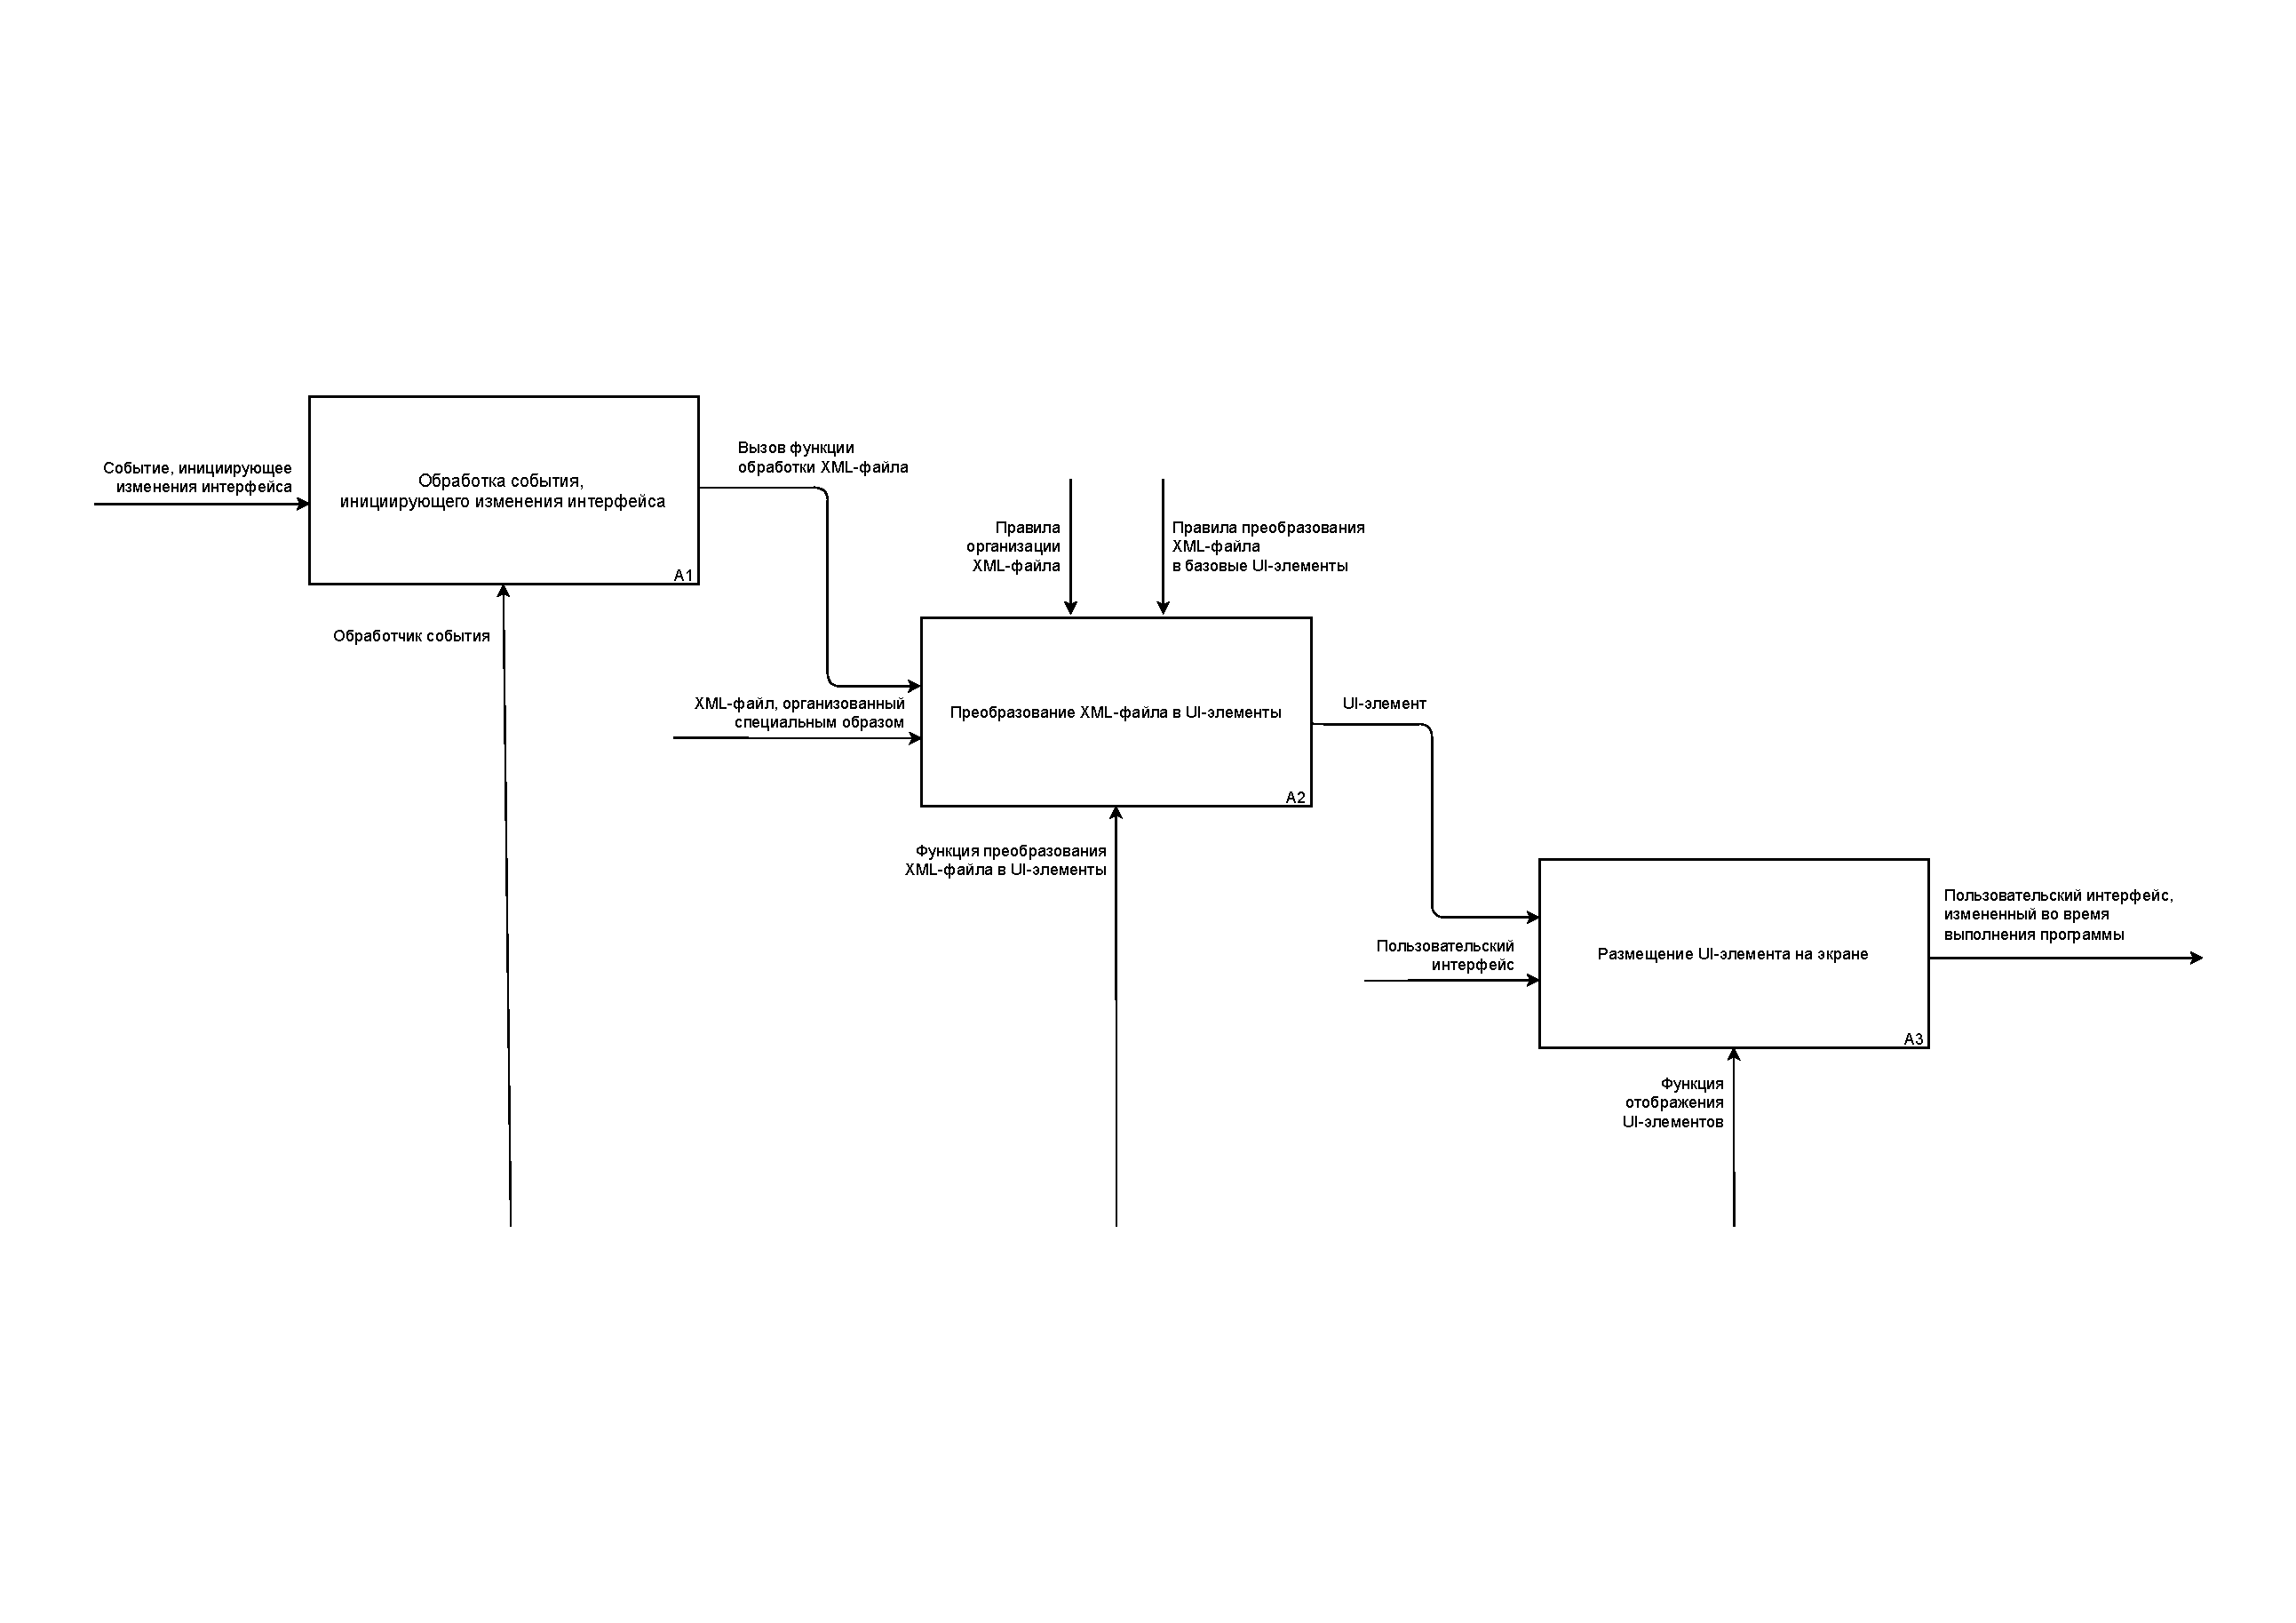
\includegraphics[scale=0.4]{img/A1.pdf}
	\caption{IDEF0~--~диаграмма уровня А1}
	\label{fig:a1}
\end{figure}

\subsection{Схемы алгоритмов}

На \textbf{первом} этапе необходимо обработать событие, которое станет инициатором изменения интерфейса.
Данным событием может стать нажатие определенного сочетания клавиш.
Каждый проектируемый экран приложения должен быть связан с конкретным XML--файлом и заранее внесен в список наблюдаемых объектов. 
По свершении события происходит вызов функции обработки XML--файла для каждого такого экрана.


На \textbf{втором} этапе происходит обработка XML--файла. 
Для этого файл должен быть организован определенным образом, чтобы в дальнейшем функция обработки корректно распознавала UI--элементы, являющиеся базовыми для платформы: первый тег XML--файла содержит в себе название базового элемента и все его необходимые свойства и их значения (название свойства и значение разделяет знак равенства <<=>>, значение заключается в кавычки <<``''>>), второй тег содержит название базового элемента.
Для создания вложенности элементов среди свойств элемента--родителя необходимо указать теги дочернего элемента.
Разметка для дочернего элемента в данном случае задается по правилам, аналогичным правилам создания родительского элемента.

Например, чтобы в нативной разработке iOS получить UILabel, занимающий 100\% площади экрана и содержащий слово <<Hello>>, расположенное по левому краю, необходимо добавить в XML--файл разметку, представленную в листинге 1.

\begin{lstlisting}[caption={Разметка XML--файла для UILabel}]
<UILabel
    width="100%"
    height="100%"
    textAlignment="left"
    text="Hello">
</UILabel>
\end{lstlisting}

В рамках данного этапа происходит получение содержимого XML--файла, разделение файла на строки для получения списка его компонентов.
Далее происходит создание корневого представления, на котором будут размещены все элементы, полученные в ходе обработки компонентов XML--файла.
После чего корневое представление и компоненты передаются в функцию преобразование элементов XML--разметки в UI--элементы.
Для корректной работы функции необходимо иметь список всех базовых UI--элементов, с которыми предполагается взаимодействие метода, а также список свойств и атрибутов для каждого элемента.
Алгоритмы работы функций представлены на рисунках \ref{fig:createLayout} ---  \ref{fig:createView}.  

Для второго этапа входным параметром XML--файл, организованный специальным образом, выходным --- UI-элемент, включающий все представления, описанные в XML--файле.

\begin{figure}[!htb]
	\centering
	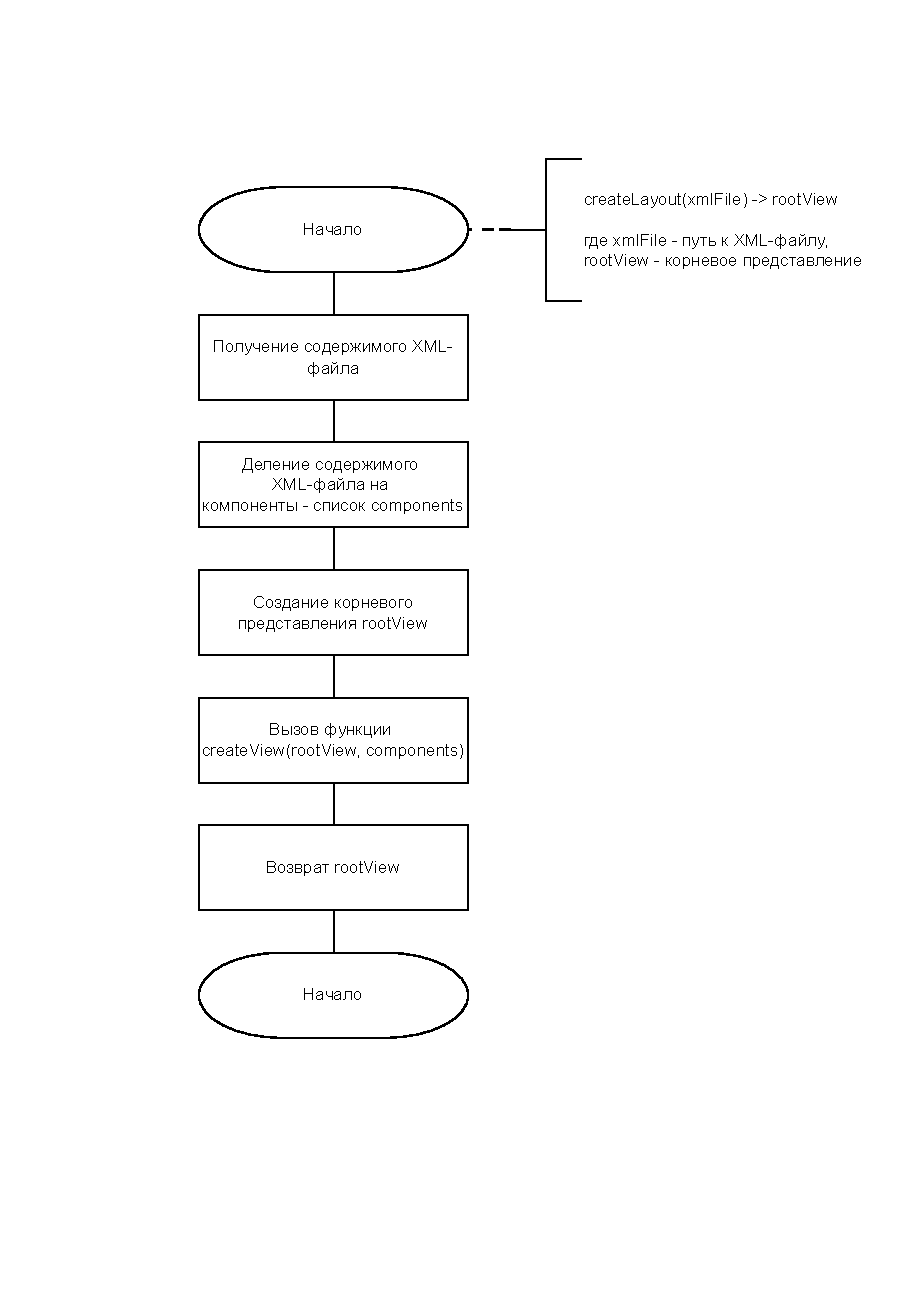
\includegraphics[scale=0.7]{img/createLayout.pdf}
	\caption{Алгоритм функции создания представления, содержащего описанные в XML--файле элементы}
	\label{fig:createLayout}
\end{figure}

\begin{figure}[!htb]
	\centering
	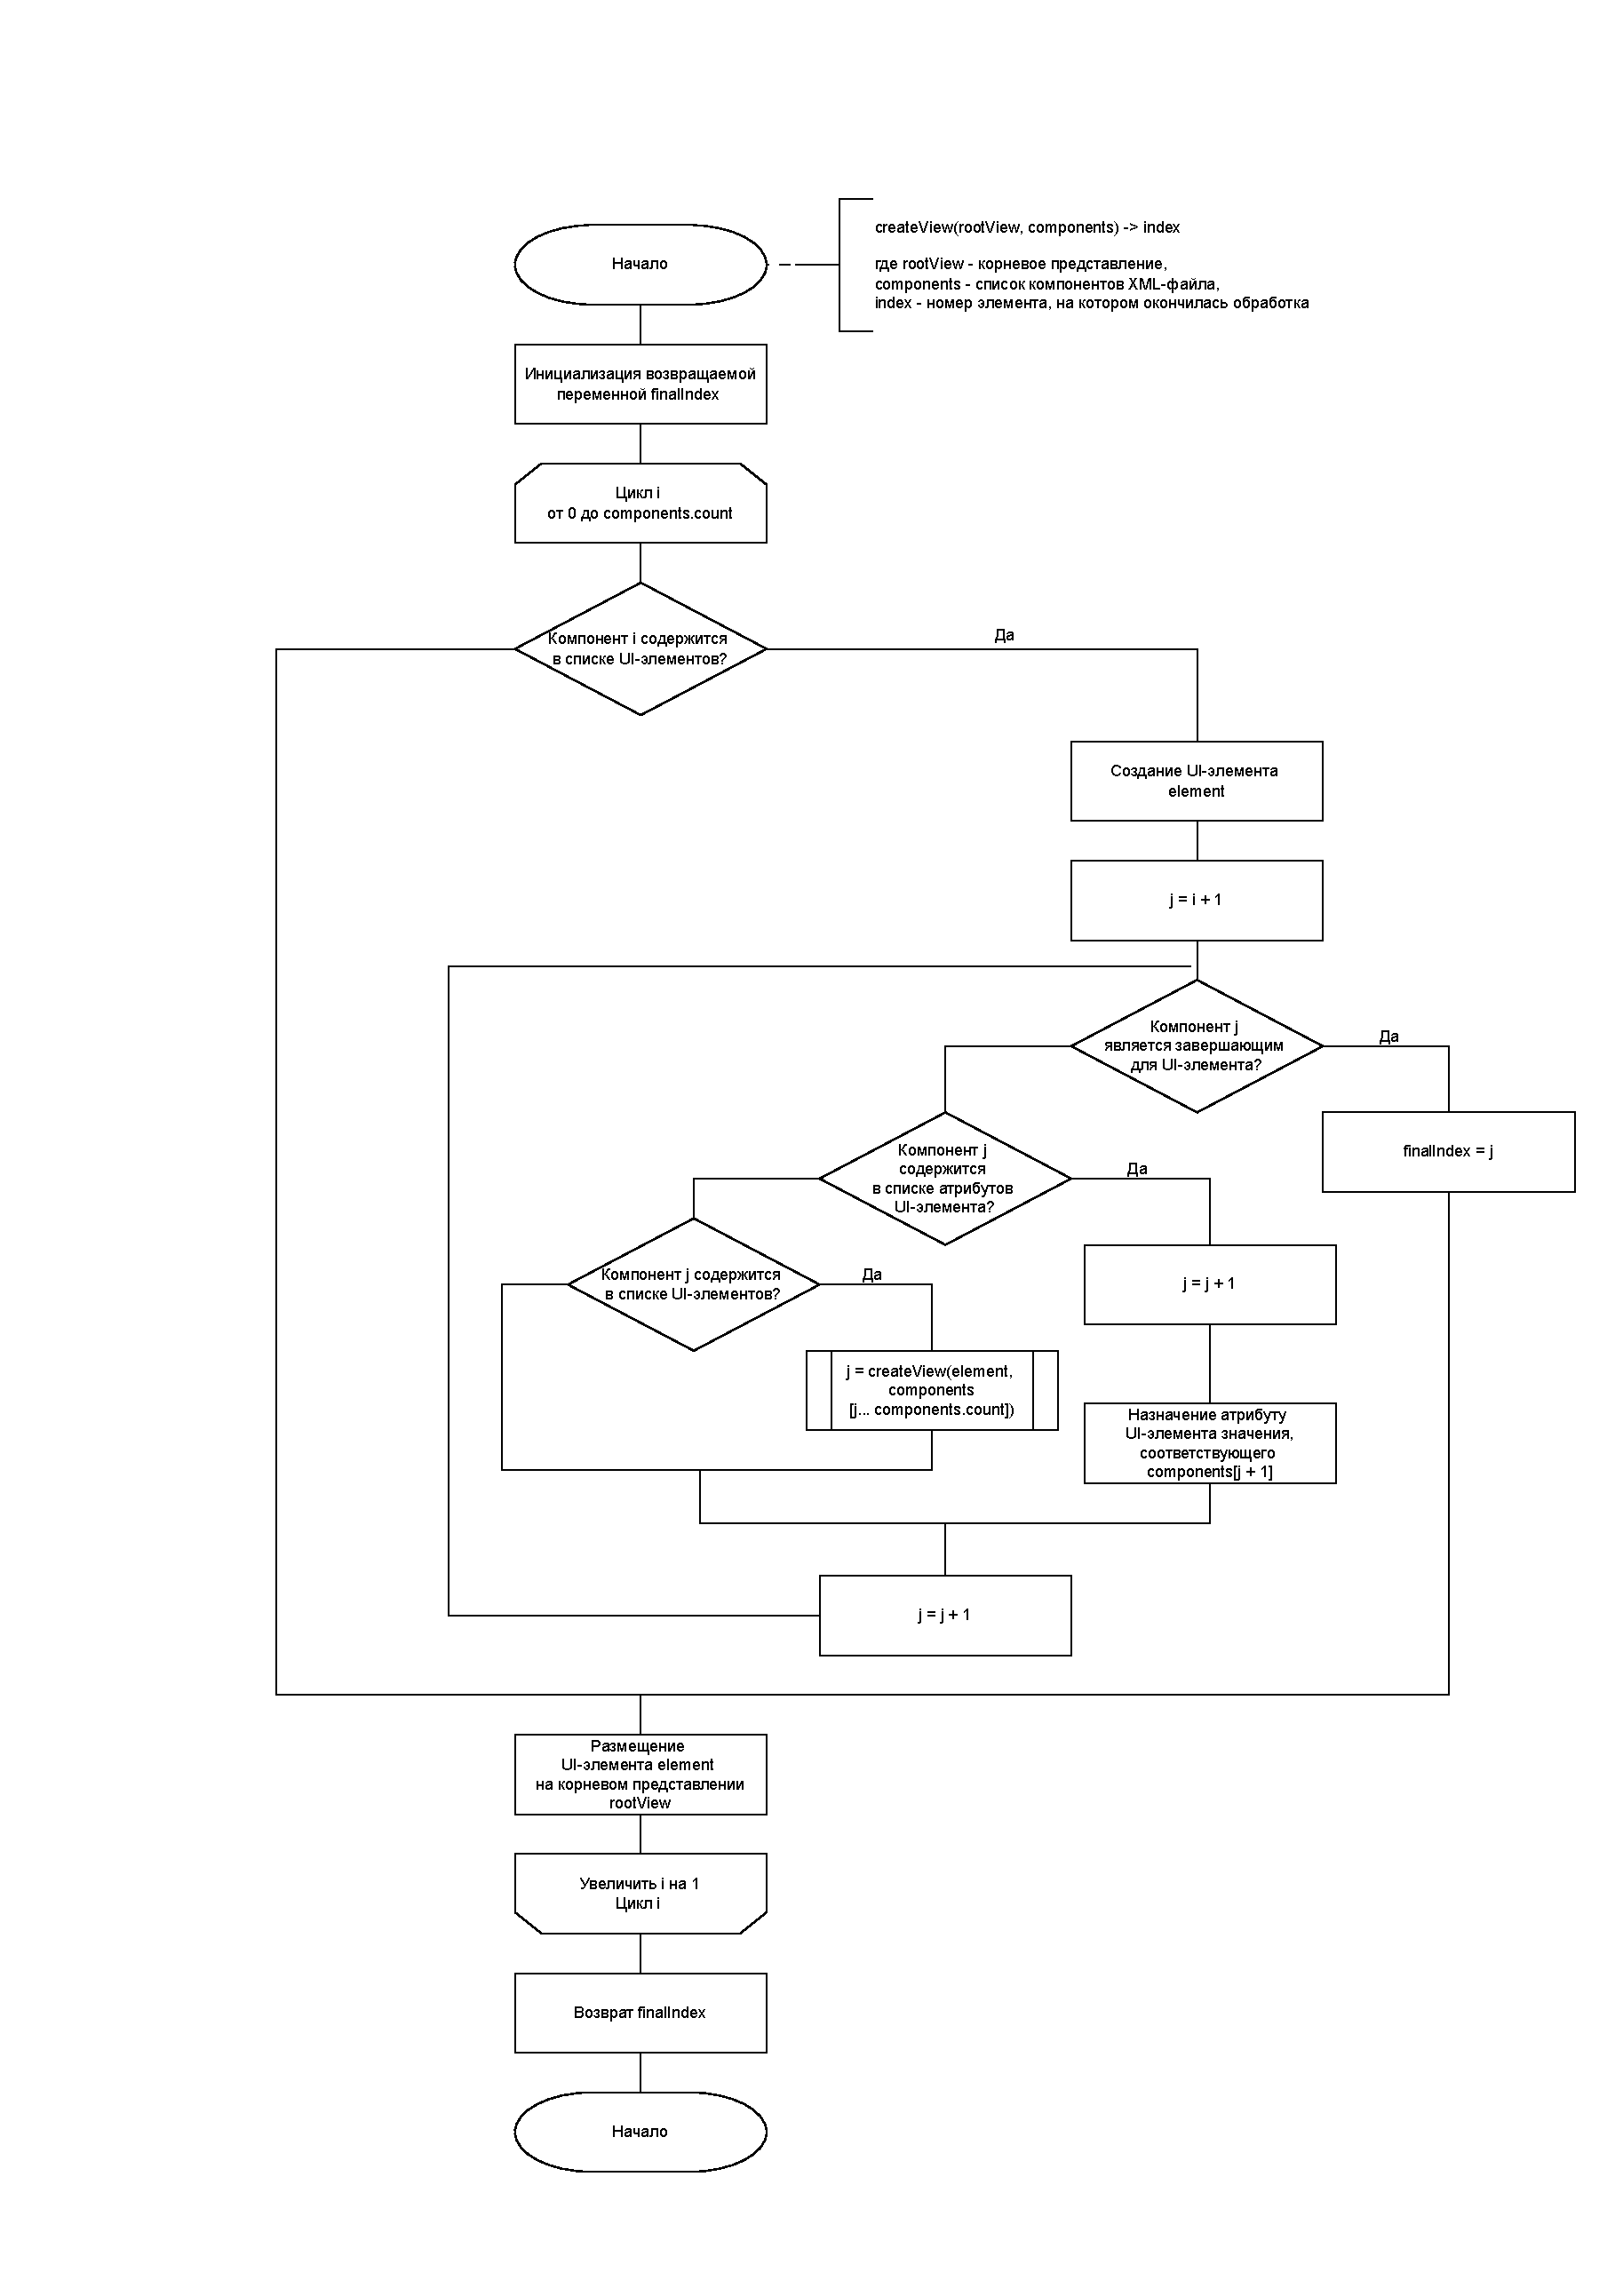
\includegraphics[scale=0.5]{img/createView.pdf}
	\caption{Алгоритм функции создания представлений}
	\label{fig:createView}
\end{figure}

\pagebreak
На \textbf{третьем} этапе происходит размещение полученного UI--элемента на экране. 
Для корректного отображения обновлений данный этап должен быть включен в жизненный цикл корневого представления экрана.


\subsection*{Вывод}

В данном разделе были сформулированы требования и ограничения к разрабатываемому методу. 
Разработан метод динамического отображения изменений пользовательского интерфейса на основе обработки изменений XML--файла.
Описаны основные этапы разработки в виде детализированной диаграммы IDEF0 и схем алгоритмов, а также изложены особенности разработанного метода. 

\pagebreak